\chapter{Phenotypic variation and resemblance between relatives.}

\newthought{The distinction between genotype and phenotype} is one of the most useful ideas in Biology.\cite{Johannsen:1911} 
The genotype of an individual (the genome), for most purposes, is decided when
the sperm fertilizes egg. The phenotype of an individual represents any
measurable aspect of an organism. Your height, to the amount of
RNA transcribed from a given gene, to what you ate last Tuesday; all
of these are phenotypes.  Nearly any phenotype we can choose to measure about an organism represents the outcome of the information encoded by their genome played out through an incredibly complicated
developmental, and physiological or behavioural processes which interact with a myriad of environmental and
stochastic factors. Honestly it boggles the mind how organisms work
as well as they do, let alone that you managed to eat lunch last Tuesday. 

\begin{marginfigure}
\begin{center}
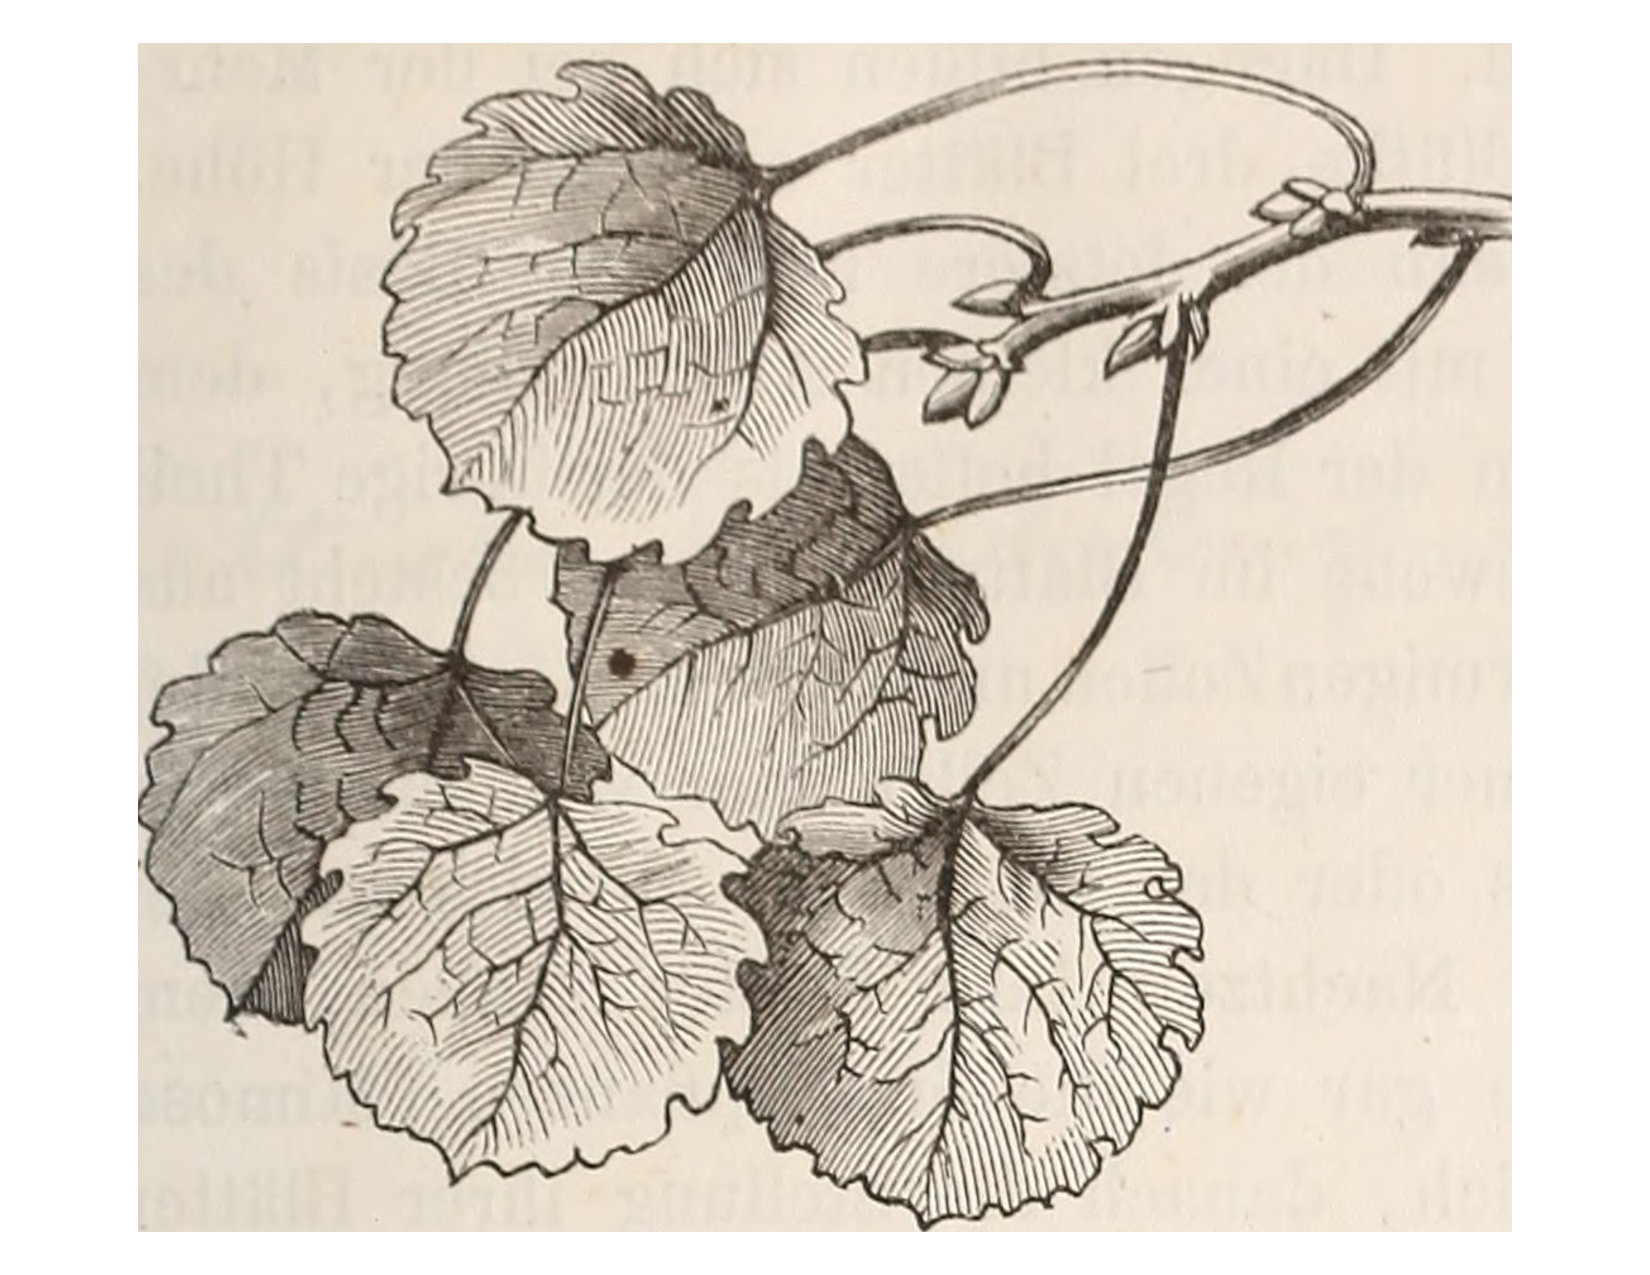
\includegraphics[width=0.8 \textwidth]{illustration_images/Quant_gen/Aspen_budset/Aspen_leaves.pdf}
\end{center}
\caption{{\it P. tremula}. Der baum. H. Schacht. 1860. BHL } \label{fig:Apsen_geno_pheno}
\end{marginfigure}

There are many different ways to think about studying the path from genotype through to phenotype. The one we will take here is to think about how phenotypic variation among individuals in a population arises as a result of genetic variation in the population.  One simples way to measure the genotype-phenotype relationship is the calculate the phenotypic mean for each genotype at a locus. For example, \citet{wang:18} explored the genetic basis of budset time in European aspen  ({\it Populus tremula}), the effect
of a specific SNP on the phenotype is shown in
in Figure \ref{fig:Apsen_geno_pheno}. Budset timing is a key trait underlying local adaptation to varying growing season length. The SNP
falls in the gene (PtFT2) that is known to play a strong role in flowering
time regulation in other plants. 
\begin{marginfigure}
\begin{center}
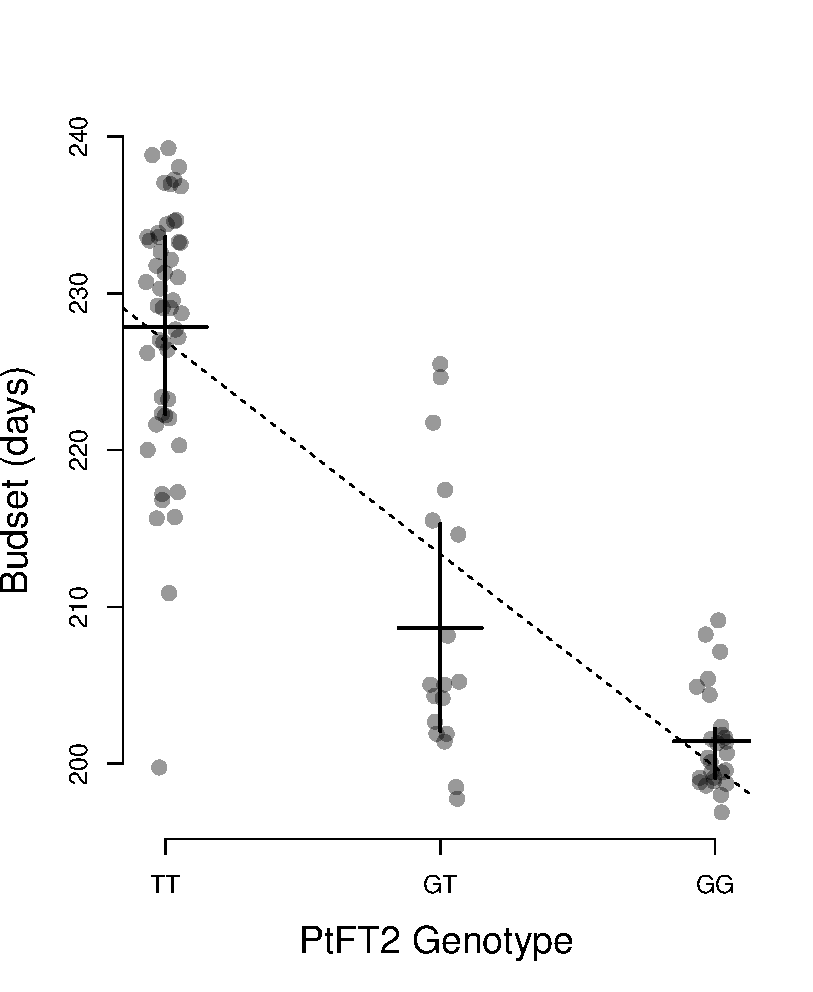
\includegraphics[width=\textwidth]{Journal_figs/Quant_gen/Wang_GWAS_poplar/Poplar_Aspen_budset_geno_pheno.pdf}
\end{center}
\caption{The effect of a flowering time gene (PtFT2) SNP on budset time in European aspen. Each dot gives the genotype-phenotype combination for
  an individual. The horizontal lines give the budset mean for each
  genotype, the vertical lines show the inter-quartile range. The
  dotted line gives the linear regression of phenotype on genotype.
  Thanks to P{\"a}r Ingvarsson for the data. } \label{fig:Apsen_geno_pheno}
\end{marginfigure}



One way for us to assess the relationship between
genotype phenotype is to fit a linear regression, i.e. the best fitting linear line through the data, of
phenotype on genotype. The slope of this line has the interpretation of being the average
effetc of substituting a copy of allele $2$ for a copy of allele
$1$. In our Aspen example the slope is $-13.6$, i.e. swopping a single $T$ for a $G$ allele
moves the budset forward by $13.6$ days, with the $GG$ homozygote
is predicted to set buds $27.2$ days earlier than the $TT$ homozygote.   


As a measure of significance of this relationship we can
calculate the p-value of this regression. To try and identify loci
that are associated with our trait genome-wide we can conduct this
regression at each SNP in the genome. One common way to display these
reuslts is to plot the logarithm of the p-value for each SNP along
genome (a so-called Manhattan plot). Here's one from 
\citet{wang:18} for their Aspen budset phenotype


\begin{figure}
\begin{center}
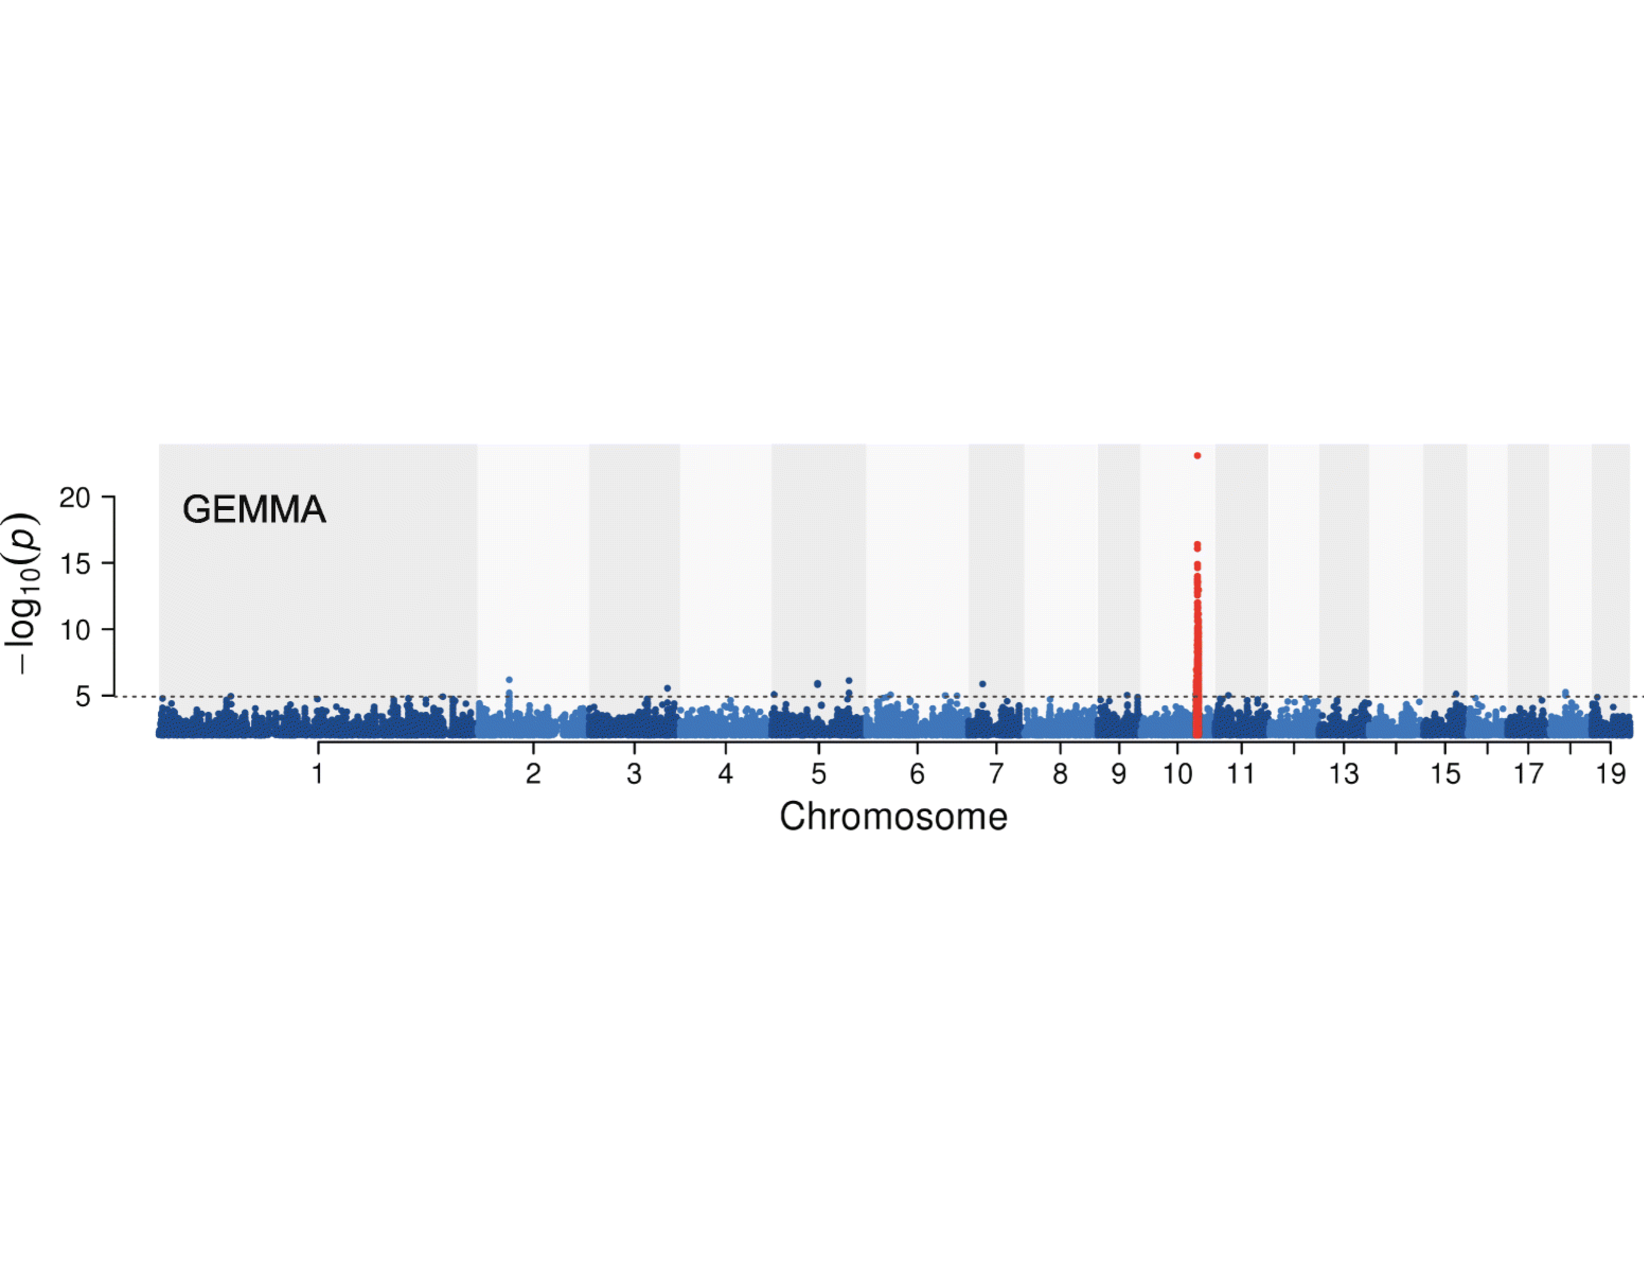
\includegraphics[width=\textwidth]{Journal_figs/Quant_gen/Wang_GWAS_poplar/Wang_Fig_just_Manhattan.pdf}
\end{center}

\caption{Manhattan plot of the p-value of the linear association
  between genotype and budset in Aspen. Each dot represents the test at a single SNP,
  plotted at physical coordinate on the genome. Different chromosomes
  are plotted in alternating colours. The SNPs surrounding the PtFT2
  gene are shown in red.} \label{fig:Apsen_Manhattan}
\end{figure}
The SNP with the most significant p-value is the PtFT2 SNP. Note
that other SNPs in the surrounding region also light up as showing a
significant association with budet timing. This is because loci that are in LD with a functional locus may in turn show an
association, not because they directly affect the phenotype but simply
because  the genotypes at the two loci are themselves are non-randomly
associated. Here is a zoomed in version (Figure 2 in \citet{wang:18}) with SNPs coloured by the
strength of their LD with the putatively functional SNP
\begin{figure}
\begin{center}
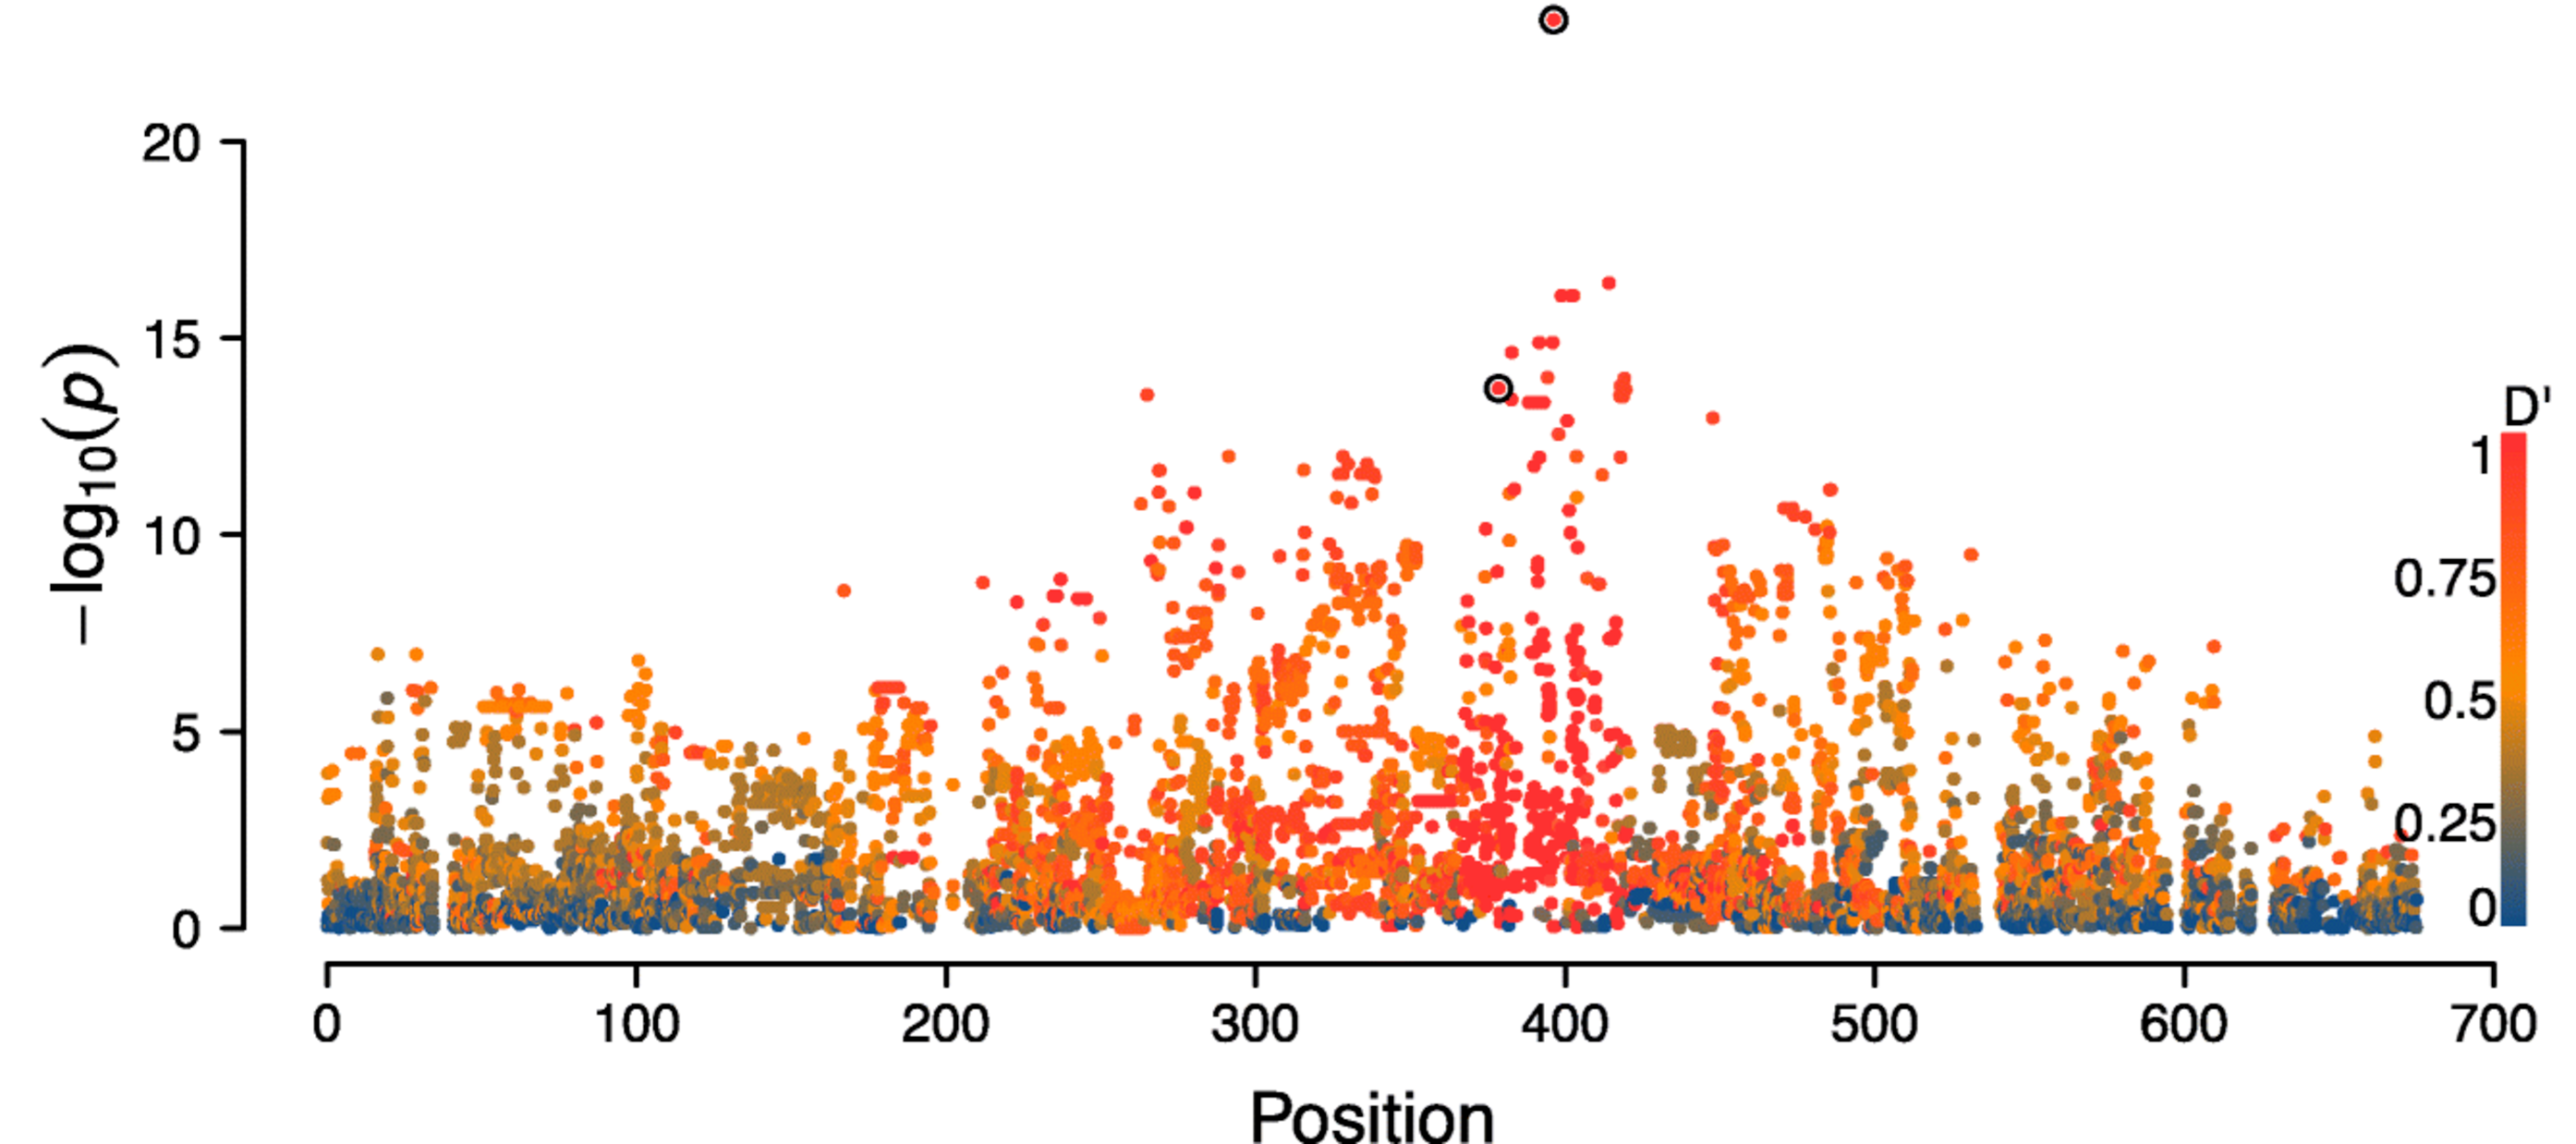
\includegraphics[width=\textwidth]{Journal_figs/Quant_gen/Wang_GWAS_poplar/Wang_Fig_zoomed_Manhattan.pdf}
\end{center}
\caption{The Manhattan plot zoomed in on the top-hit (red SNPs from Figure
  \ref{fig:Apsen_Manhattan}). SNPs are now coloured by their $D\prime$
  value with the most significant SNP. $D\prime$ is the $D$ LD
  covariance between a pair of loci ($D$, eqn \gc{XXX}) normalized by
  the largest value it can take given the allele frequencies. From
  Figure 2 of } \label{fig:Apsen_zoom_Manhattan}
\end{figure}
Note how SNPs with strong LD with the functional allele (redder
points) have more significant p-values. 

Variation in some traits seems to have a relatively simple genetic
basis. In our Aspen example there is one clear large-effect locus,
which explains  62\% of the variation in budset. \marginnote{
``All that we mean when we speak of a gene [allele] for pink eyes is, a gene which differentiates a pink eyed fly 
from a normal one — not a gene [allele] which produces pink eyes per se, for the character pink eyes is dependent 
on  the action of many other genes." - \citet{sturtevant:15}
} Note that even in this case where we have an allele with a very strong effect on a phenotype this is not an allele {\it for} budset, nor is the locus it falls in a gene {\it for} budset. It is an allele that is associated with budset in the current set of environments. In a different set of environments this allele's affects may be far smaller, and a different set of alleles may contribute to phenotype variation. The gene it falls close to is just one of many genes and molecular pathways involved in budset, a mutant screen for budset may uncover many genes with larger effect, this gene is just a locus that happens to be polymorphic in this particular set of populations. 

While phenotypic variation in some phenotypes has a relatively simple genetic basis, many phenotypes are likely much more genetically complex in their
variation involving the functional effect of many alleles at hundreds or thousands of polymorphic loci. Such genetically complex traits are called polygenic traits. 

In this chapter we will use our understanding of the sharing of alleles between relatives to understand the phenotypic resemblance between relatives in
quantitative phenotypes. This will allow us to understand the contribution of genetic variation to phenotypic variation. In the next chapter we then use these results to understand the evolutionary change in quantitative phenotypes in response to selection. \\

\subsection{A simple additive model of a trait}
Let's imagine that the genetic component of the variation in our trait is controlled by $L$ autosomal loci that act in an additive manner. The frequency of allele $1$ at locus $l$ is $p_l$, with each copy of allele $1$ at this locus increasing your trait value by $a_l$ above the population mean.
The phenotype of an individual, let's call her $i$, is $X_i$.
Her genotype at SNP $l$, is
$G_{i,l}$. Here $G_{i,l}=0,~1,$ or $2$  represents the number of copies of allele $1$ she
has at this SNP. Her expected phenotype, given her genotype, is then
\begin{equation}
\E (X_i | G_{i,1},\cdots,G_{i,L}) =\mu + X_{A,i} = \mu+\sum_{l=1}^L G_{i,l} a_{l} \label{pheno_geno}
\end{equation}
where $\mu$ is the mean phenotype in our population, and $X_{A,i}$ is
the deviation away from the mean phenotype due to her genotype. Now in reality the genetic phenotype is a function of the
expression of those alleles in a particular environment. Therefore, we
can think of this expected phenotype as being an average across a set
of environments that occur in the population. \\

%\gc{NEED to resolve $\mu$ in above equation}


When we measure our individual's observed phenotype we see
\begin{equation}
X_i =   \mu+X_{A,i} + X_{E,i} \label{pheno_geno_environ}
\end{equation}
where $X_E$ is the deviation from the mean phenotype due to the
environment. This $X_E$ included the systematic effects of the environment
our individual finds herself in and all of the noise during
development, growth, and the various random insults that life throws
at our individual. If a reasonable number of loci contribute to
variation in our trait then we can approximate the distribution of
$X_{A,i}$ by a normal distribution due to the central limit theorem (see Figure \ref{fig:QT1}). Thus if we can
approximate the distribution of the effect of environmental variation
on our trait ($X_{E,i}$) also by a normal distribution, which is
reasonable as there are many small environmental effects, then the
distribution of phenotypes within the population ($X_i$) will be
normally distributed (see Figure \ref{fig:QT1}).\\

\begin{figure}
\begin{center}
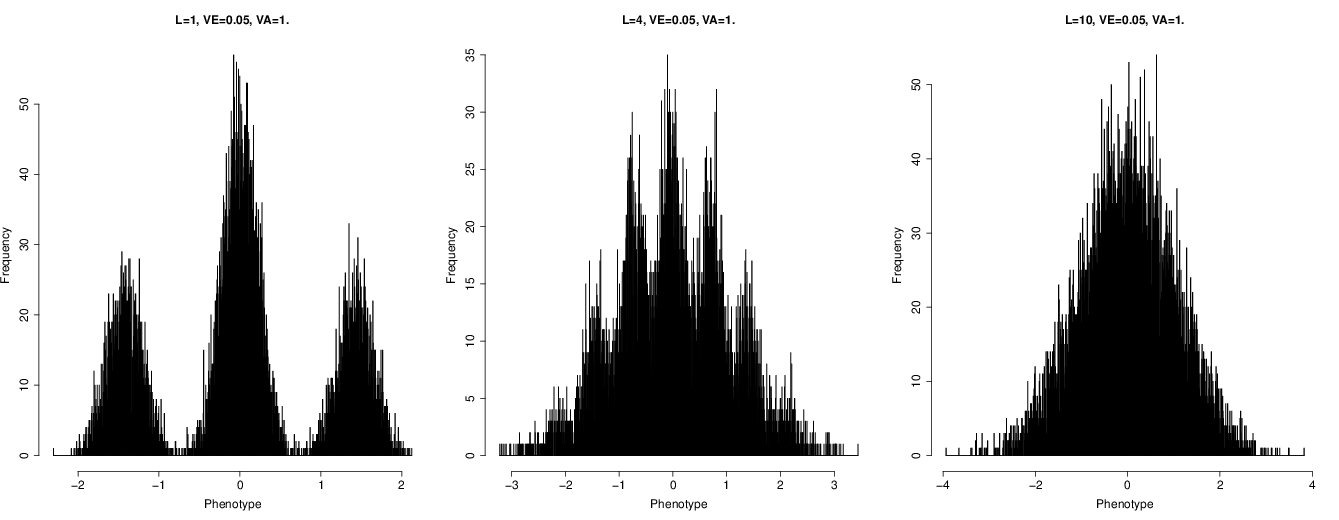
\includegraphics[width=\textwidth]{figures/QT1.png}
\end{center}
\caption{The convergence of the phenotypic distribution to a normal
  distribution. Each of the three histograms shows the distribution of
the phenotype in a large sample, for increasing large numbers of loci ($L$). I have simulated each individual's
phenotype following equation \ref{pheno_geno} and \ref{pheno_geno_environ}. Specifically we've simulated each
individuals biallelic genotype at $L$ loci, assuming Hardy-Weinberg proportions
and that the allele is at 50\% frequency. we've assume that all of the
alleles have equal effects and combine them additively together. We then add an environmental contribution, which is normally distributed with variance $0.05$. Note that in the left two pictures you can see peaks
corresponding to different genotypes; this is because we have little environmental noise in practice we can rarely see such peaks.} \label{fig:QT1}
\end{figure}


\begin{figure}
\begin{center}
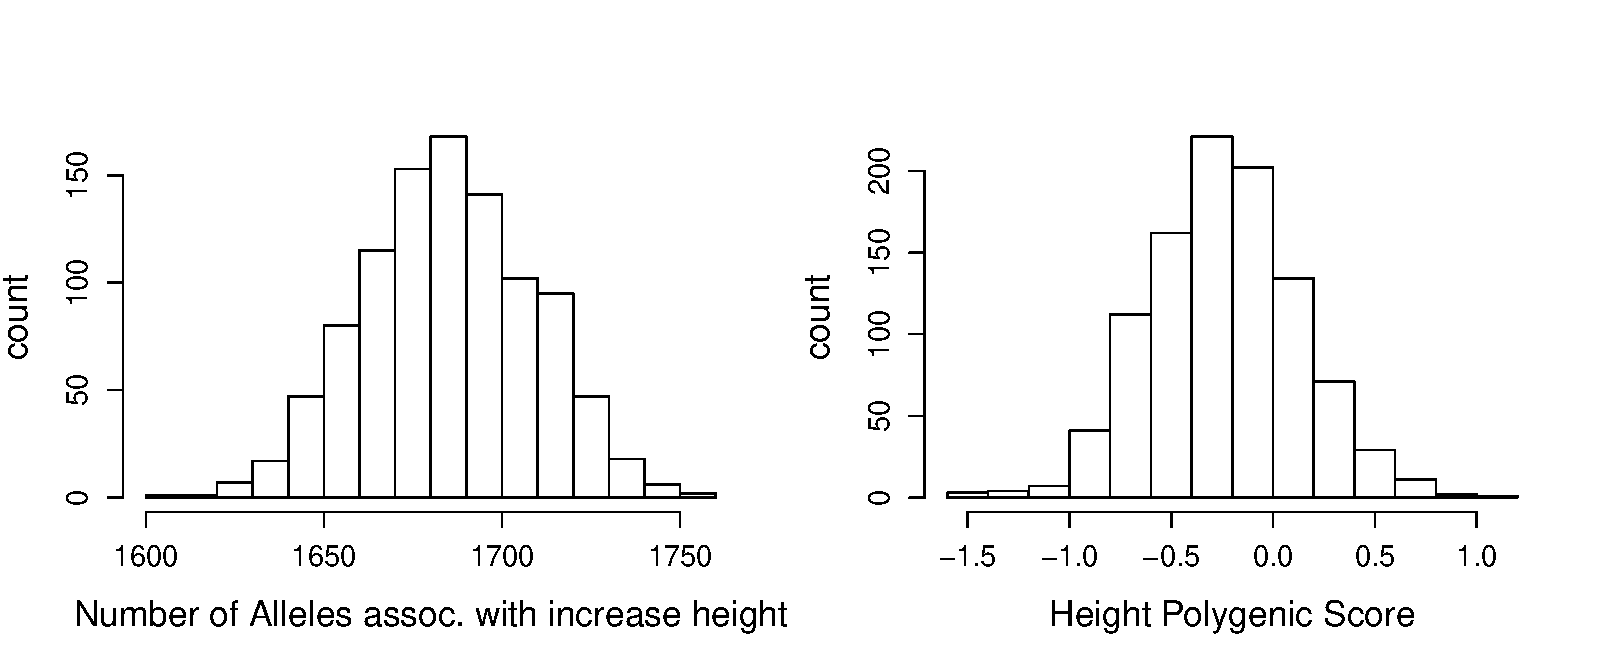
\includegraphics[width=\textwidth]{figures/Biobank_height_dist.pdf}
\end{center}
\caption{} \label{fig:QT1}
\end{figure}



Note that as this is an additive model we can decompose eqn. \ref{pheno_geno_environ} into the
effects of the two alleles at each locus, in particular we can rewrite
it as
\begin{equation}
X_i = \mu + X_{iM}+X_{iP} +X_{iE}
\end{equation}
where $X_{iM}$ and $X_{iP}$ are the contribution to the phenotype of
the allele that our individual received from her mother (maternal
alleles) and father (paternal alleles) respectively. This will come in
handy in just a moment when we start thinking about the phenotype covariance of relatives.\\

Now obviously this model seems silly at first sight as alleles don't
only act in an additive manner, as they interact with alleles at the
same loci (dominance) and at different loci (epistasis). Later we'll
relax this assumption, 
however, we'll find that if we are interested in evolutionary change
over short time-scales it is actually only the ``additive
component'' of genetic variation that will (usually) concern us. 
We will define this more formally later on, but for the moment 
we can offer the intuition that parents only get to pass on a single
allele at each locus on to the next generation. As such, it is the
effect of these transmitted alleles, averaged over possible matings,
that is an individual's average contribution  to the next generation
(i.e. the additive effect of the alleles that their genotype consists of).



\subsection{Additive genetic variance and heritability}
As we are talking about an additive genetic model we'll talk about the
additive genetic variance ($V_A$), the variance due to the additive
effects of segregating genetic variation. This is a subset of the total genetic
variance if we allow for non-additive effects. \\

The variance of our phenotype across individuals ($V$) can write this as
\begin{equation}
V = Var(X_A) + Var(X_E) = V_A+V_E
\end{equation}
in writing this we are assuming that there is no covariance between $X_{G,i}$
and $X_{E,i}$ i.e. there is no covariance between genotype and
environment. \\

Our additive genetic variance can be written as
\begin{equation}
V_A = \sum_{l=1}^L Var(G_{i,l} a_{l})
\end{equation}
where $Var(G_{i,l} a_{l})$ is the contribution to the additive
variance among individuals of the $l$ locus. Assuming random mating we
can write our additive genetic variance as
\begin{equation}
V_A = \sum_{l=1}^L a_{l}^2 2 p_l(1-p_l)
\end{equation}
where the $ 2 p_l(1-p_l)$ term follows the binomial sampling of two
alleles per individual at each locus. \\

\paragraph{The narrow sense heritability}
We would like a way to think about what proportion of the variation
in our phenotype across individuals is due to genetic differences as
opposed to environmental differences. Such a quantity will be key in
helping us think about the evolution of phenotypes. For example, if
variation in our phenotype had no genetic basis then no matter how
much selection changes the mean phenotype within a generation
the trait will not change over generations. \\

We'll call the proportion of the variance that is genetic the
heritability, and denote it by $h^2$. We can then write this as
\begin{equation}
h^2 = \frac{Var(X_A)}{V} = \frac{V_A}{V}
\end{equation}
remember that we thinking about a trait where all of the alleles act
in a perfectly additive manner. In this case our heritability $h^2$ is
referred to as the narrow sense heritability, the proportion of the
variance explained by the additive effect of our loci.
When we allow dominance
and epistasis into our model we'll also have to define the broad sense
heritability (the total proportion of the phenotypic variance
attributable to genetic variation).\\

The narrow sense heritability of a trait is a useful quantity, indeed
we'll see shortly that it is exactly what we need to understand the
evolutionary response to selection on a quantitative phenotype. We can
calculate the narrow sense heritability by using the resemblance between
relatives. For example, if our phenotype was totally environmental we
should not expect relatives to resemble each other any more than random
individuals drawn from the population. Now the obvious caveat here is
that relatives also share an environment, so may resemble each other
due to shared environmental effects. \\

\subsection{The covariance between relatives}
So we'll go ahead and calculate the covariance in phenotype between two individuals
($1$ and $2$) who have a phenotype $X_1$ and $X_2$ respectively.
\begin{equation}
Cov(X_1,X_2) =
Cov\left((X_{1M}+X_{1P}+X_{1E}),((X_{2M}+X_{2P}+X_{2E}) \right)
\end{equation}
We can expand this out in terms of the covariance between the various
components in these sums.\\

To make our task easier we (and most analyses) will assume two things
\begin{enumerate}
\item that we can ignore the covariance of the environments
between individuals (i.e. $Cov(X_{1E},X_{2E})=0$)
\item that we can ignore the covariance
between the environment variation experience by an individual and the
genetic variation in another individual (i.e. $Cov(X_{1E},(X_{2M}+X_{2P}))=0$).
\end{enumerate}

The failure of these assumptions
to hold can severely undermine our estimates of heritability, but we'll
return to that later. Moving forward with these assumptions, we can
write our phenotypic covariance between our pair of individuals as
\begin{equation}
Cov(X_1,X_2) =
Cov((X_{1M},X_{2M})+Cov(X_{1M},X_{2P})+Cov(X_{1P},X_{2M})
+Cov(X_{1P},X_{2P}) \label{cov_rels_1}
\end{equation}
This is saying that under our simple additive model we can see the
covariance in phenotypes between individuals as the covariance between
the allelic effects in our individuals. We can use our results about
the sharing of alleles between relatives to obtain these terms.
But before we write down the general case lets quickly work through some
examples. \\


\paragraph{The covariance between Identical Twins}
Lets first consider the case of a pair of identical twins from two
unrelated parents. Our pair of twins share their maternal and paternal
allele identical by descent ($X_{1M}=X_{2M}$ and $X_{1P}=X_{2P}$). As their maternal and
paternal alleles are not correlated draws from the population,
i.e. have no probability of being $IBD$ as we've said the parents are unrelated, the
covariance between their effects on the phenotype is zero  
(i.e. $Cov(X_{1P},X_{2M})=Cov(X_{1M},X_{2P})=0$). In that case
eqn. \ref{cov_rels_1} is
\begin{equation}
Cov(X_1,X_2) = Cov((X_{1M},X_{2M})+Cov(X_{1P},X_{2P}) = 2Var(X_{1M})
= V_A
\end{equation}
Now in general identical twins are not going to be super helpful for
us in estimating $h^2$ as under models with non-additive effects
identical twins have higher covariance than we'd expect as they
resemble each other also because of the dominance effects as they
don't just share alleles they share their entire genotype.\\

\paragraph{The covariance in phenotype between mother and child}.

\begin{marginfigure}
\begin{center}
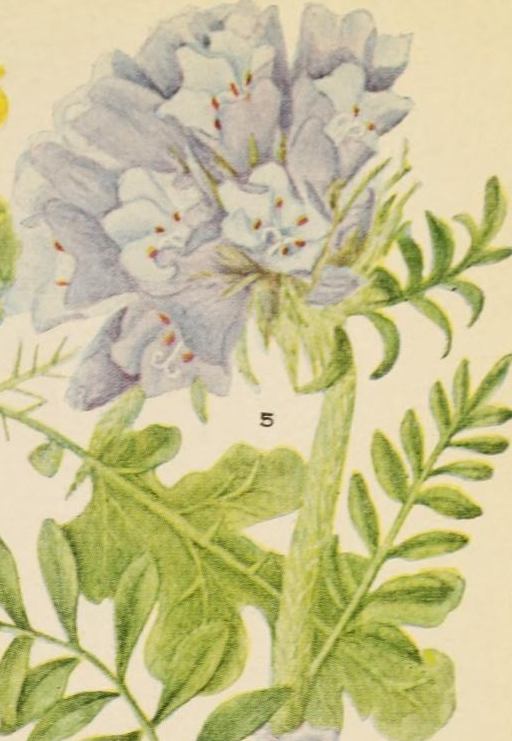
\includegraphics[width=0.5\textwidth]{illustration_images/Quant_gen/Polemonium_viscosum_Galen/Polemonium_viscosum.jpg}
\end{center}
\caption{{\it Plemonium viscosum.}  Modified from Flowers of Mountain and Plain. New York :H.W. Wilson Co.,1920. \href{https://www.flickr.com/photos/biodivlibrary/8220461305/in/album-72157632108046380/}{BHL}. }
\end{marginfigure}

\marginnote{
\begin{question}
Galen \cite{galen:96} explored selection on flower shape in
{\it P. viscosum}.  She found that plants with larger  corolla flare
had more bumblebee visits, which resulted in higher seed set and a
$17\%$ increase in corolla flare in the plants contributing to the
next generation. Based on the data in Fig. \ref{fig:Galen_corolla}
what is the expected response in the next generation? 
\end{question}
}

\begin{marginfigure}
\begin{center}
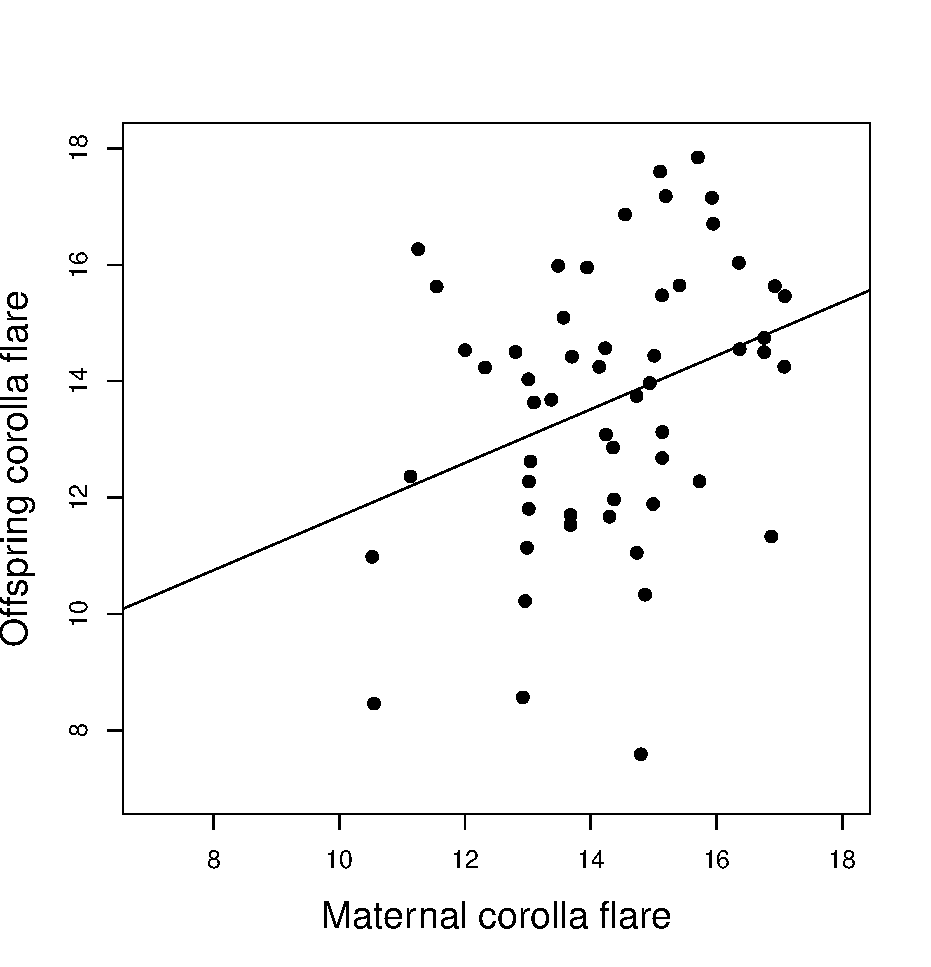
\includegraphics[width=\textwidth]{Journal_figs/Quant_gen/Galen_flower_herit/Galen_corolla_flare.pdf} 
\end{center}
\caption{The relationship between maternal and offspring corolla flare (flower
  width) in P. viscosum. Redrawn from \citeauthor{galen:96}.} \label{fig:Galen_corolla}  %
\end{marginfigure}


If the mother and father are unrelated individuals (i.e. are two
random draws from the population) then the mother and a child share
one allele IBD at each locus (i.e. $r_1=1$ and $r_0=r_2=0$). Half the
time our mother transmits her paternal allele to the child, in which
case $X_{P1}=X_{M2}$ and so $Cov(X_{P1},X_{M2})=Var(X_{P1})$ and all
the other covariances in eqn. \ref{cov_rels_1} zero, and half
the time she transmits her maternal allele to the child
$Cov(X_{M1},X_{M2})=Var(X_{M1})$ and all the other terms zero. By this
argument $Cov(X_1,X_2) = \half Var(X_{M1}) + \half Var(X_{P1}) = \half
V_A$. \\

\paragraph{The covariance between general pairs of relatives under an
additive model}

\marginnote{
\begin{question}
{\bf A)} In polygynous blackbird populations (i.e. males mate with
several females), paternal half-sibs can be identified.  Suppose that
the covariance of tarsus lengths among half-sibs is 0.25 $cm^2$ and
that the total phenotypic variance is 4 $cm^2$.  Use these data to
estimate $h^2$ for tarsus length in this population. \\

{\bf B)} Why might paternal half-sibs be preferable for measuring
heritability than maternal half-sibs? 
\end{question}
}


The two examples make clear that to understand the covariance between
phenotypes of relatives we simply need to think about the alleles they
share IBD. Consider a pair of relatives ($1$ and $1$) with a probability $r_0$,
$r_1$, and $r_2$ of sharing zero, one, or two alleles IBD
respectively. When they share zero alleles
$Cov((X_{1M}+X_{1P}),(X_{2M}+X_{2P}))=0$, when they share one allele
$Cov((X_{1M}+X_{1P}),(X_{2M}+X_{2P}))=
Var(X_{1M})=\frac{1}{2}V_A$, and when they share two alleles $Cov((X_{1M}+X_{1P}),(X_{2M}+X_{2P}))=
V_A$. Therefore, the general covariance between two
relatives is
\begin{equation}
Cov(X_1,X_2) = r_0 \times 0 + r_1 \frac{1}{2}V_A + r_2  V_A =
2 F_{1,2} V_A  \label{additive_covar_general_rellys}
\end{equation}\\
So under a simple additive model of the genetic basis of a phenotype
to measure the narrow sense heritability we need to measure the
covariance between a set of pairs of relatives (assuming that we can remove the effect of
shared environmental noise). From the covariance between relatives we
can calculate $V_A$, we can then divide this by the total phenotypic
variance to get $h^2$. \\
%One way potentially to get somewhat around the
%shared environmental effect is to use paternal half-sibs as they share a

Another way that we can estimate the narrow sense heritability is
through the regression of child's phenotype on the parental mid-point
phenotype. The parental mid-point phenotype is simple the average of
the mum and dad's phenotype. Denoting the child's phenotype by $X_{kid}$ and mid-point
phenotype by $X_{mid}$ so that if we take the regression $X_{kid} \sim X_{mid}$ this
regression has slope $\beta = Cov(X_{kid},X_{mid})/Var(X_{mid})$.
The covariance of $Cov(X_{kid},X_{mid})=\half
V_A$, and $Var(X_{mid}) = \half V$ as by taking the average of the
parents we have halved the variance, such that the slope of the
regression is
\begin{equation}
\beta_{mid,kid}= \frac{Cov(X_{kid},X_{mid})}{Var(X_{mid})} = \frac{V_A}{V} = h^2
\end{equation}
i.e. the regression of the child's phenotype on the parental midpoint
phenotype is an estimate of the narrow sense heritability. This is a
common way to estimate heritability, although it doesn't bypass the
need to control for environmental correlations between relatives. \\

Our regression allows us to attempt to predict the phenotype of the
child given the phenotypes of the parents; how well we can do this depends on the
slope. If the slope is close to zero then the parental phenotypes hold no
information about the phenotype of the child, while if the slope is
close to one then the parental mid-point is a good guess at the child's
phenotype.\\
\begin{figure}
\begin{center}
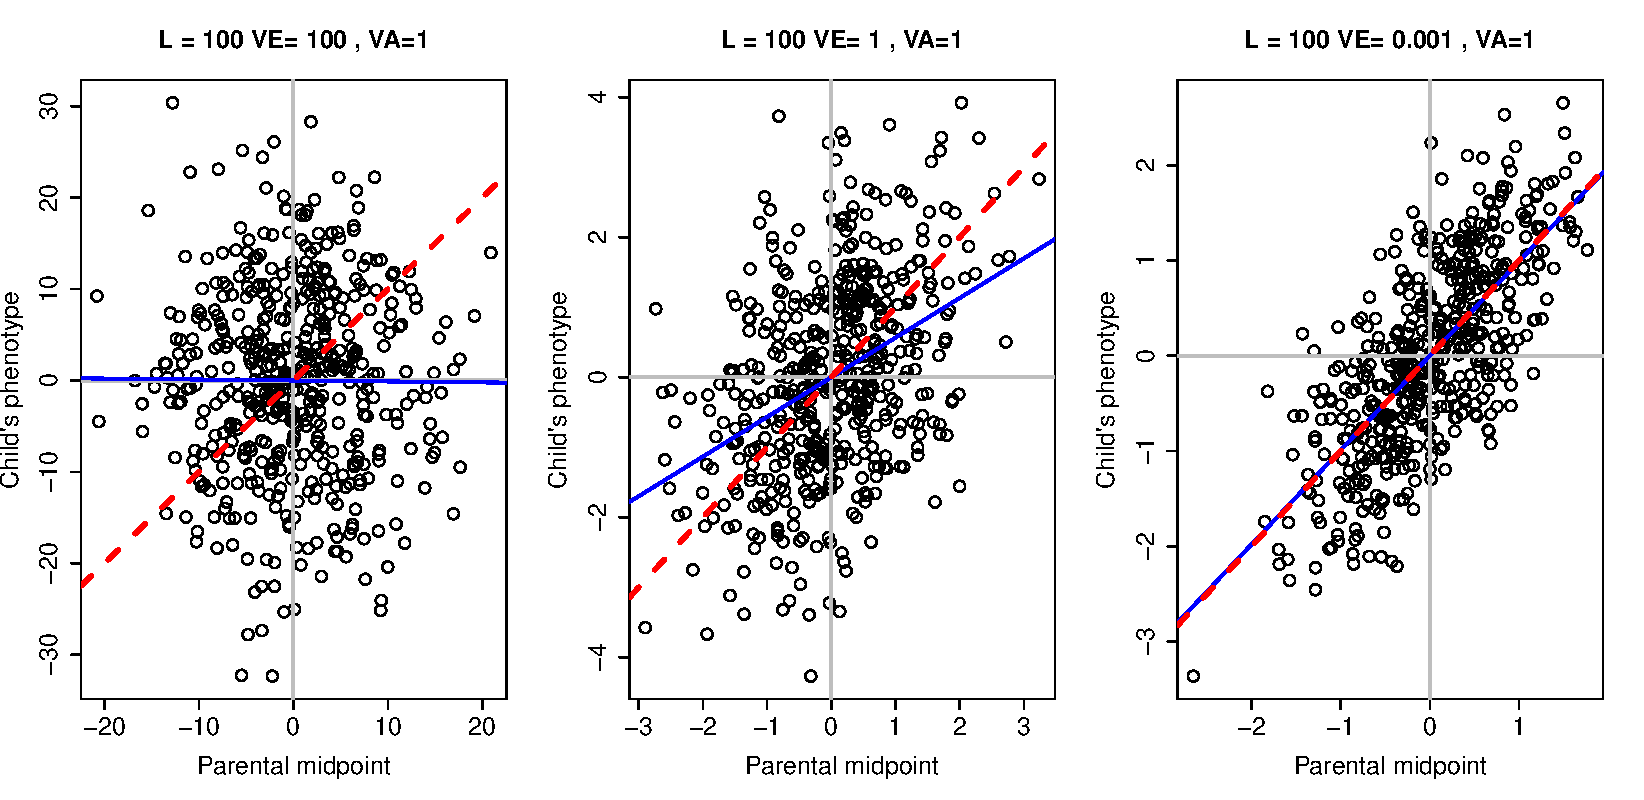
\includegraphics[width=\textwidth]{figures/QT2.pdf}
\end{center}
\caption{Regression of parental mid-point phenotype on child's
  phenotype. The three panels show decreasing levels of environmental
  variance ($V_E$) holding the additive genetic variance constant ($V_A=1$). 
 In these figures we simulate $100$ loci, as described in
 the caption of Figure \ref{fig:QT1}.WeI simulate the genotypes and
 phenotypes of the two parents, and then simulate the child's genotype
following mendelian transmission. The blue line shows $x=y$ the red
line shows the best fitting linear regression line. }
\end{figure}

More formally the expected phenotype of the child given the parental
phenotypes is
\begin{equation}
\E(X_{kid} | X_{mum},X_{dad}) = \mu +
\beta_{mid,kid}(X_{mid} - \mu) =\mu + h^2(X_{mid} - \mu)  \label{predict_kid}
\end{equation}
this follows from the definition of linear regression. So to find the
child's predicted phenotype we simply take the mean phenotype and add
on the difference between our parental mid-point multiplied by our
narrow sense heritability. \\


\begin{question}
Briefly explain Galton’s observation of the regression towards
mediocrity in light of Mendelian inheritance. 
\end{question}

\paragraph{Estimating additive genetic variance across a variety of
  different relationships.}

In many natural populations we may have access to individuals of a
range of different relationships to each other (through monitoring
of the paternity of individuals), but relatively few individuals of a
given relationship (e.g. sibs). We can try and use this information as
fully as possible in a mixed model framework. Considering equation
\ref{pheno_geno_environ} we can write an individual's phenotype $X_i$
 as 
\begin{equation}
X_i =  \mu  + X_{A,i} + e_i 
\end{equation}
where $e_i \sim N(0,V_E)$ and $X_{A,i}$ is normally distributed across
individuals with covariance matrix $V_A A$ where the the entries for
a pair of individuals i and j are 
$A_{ij}= 2 F_{i,j}$ and $A_{ii}= 1$. Given the matrix $A$ we can estimate $V_A$. We can
also add fixed effects into this model to account for generation
effects, additional mixed effects could also be included to account
for shared environments between particular individuals (e.g. a shared nest).
This is sometimes called the ``animal model''.



\section{Multiple traits.}

Traits often covary with each other, due to both environmentally
induced effects (e.g. due to the effects of diet on multiple traits)
and due to the expression of underlying genetic covariance between
traits. In turn this genetic covariance can reflect pleiotropy, a
mechanistic effect of an allele on multiple traits (e.g. variants that
effect skin pigmentation often effect hair color) or the genetic
linkage of loci independently affecting multiple traits. If we are
interested in evolution over short time-scales we can (often) ignore
the genetic basis of this correlation. 

Consider two traits $X_{1,i}$ and $X_{2,i}$ in an indivdual $i$, these could be
say the individual's leg length and nose length. As before we can write
these as 
\begin{eqnarray}
X_{1,i} &= \mu_1+ X_{1,A,i} + X_{1,E,i}  \nonumber \\
X_{2,i} &= \mu_2 +X_{2,A,i} + X_{2,E,i} \nonumber \\
\end{eqnarray}
As before we can talk about the total phenotypic variance ($V_1,V_2$),
environmental variance  ($V_{1,E}$ and $V_{2,E}$), and the additive genetic variance in trait one and two
($V_{1,A}$, $V_{2,A}$). But now we also have to consider the 
total covariance $V_{1,2}=Cov(X_{1},X_{2})$, the environmentally induced covariance between the traits ($V_{E,1,2}=Cov(X_{1,E}
,X_{2,E} )$) and the additive genetic covariance ($V_{A,1,2}
=Cov(X_{1,A} ,X_{2,A} )$) between trait one and two.

We can store these values in a matrices 
\begin{equation}
\bf{V}= \left( \begin{array}{cc} 
V_{1} & V_{1,2} \\
V_{1,2} & V_{2} \\
\end{array} \right) \label{P_matrix}
\end{equation}
and
\begin{equation}
\bf{G}= \left( \begin{array}{cc} 
V_{1,A} & V_{A,1,2} \\
V_{A,1,2} & V_{2,A} \\
\end{array} \right)  \label{G_matrix}
\end{equation}
we can generalize this to an abitrary number of traits.

We can estimate these quantities, in a similar way to before, by
studying the covariance in different traits between relatives: 
\begin{equation}
Cov(X_{1,i},X_{2,j}) = 2 F_{i,j} V_{A,1,2}
\end{equation}

\graham{Added genetic correlation, needed for the stalk-eyed flies}

A simple example of a genetic covariance is the covariance of male and
female phenotypes. 
\graham{add question estimating genetic coar/corr}
\begin{figure}
\begin{center}
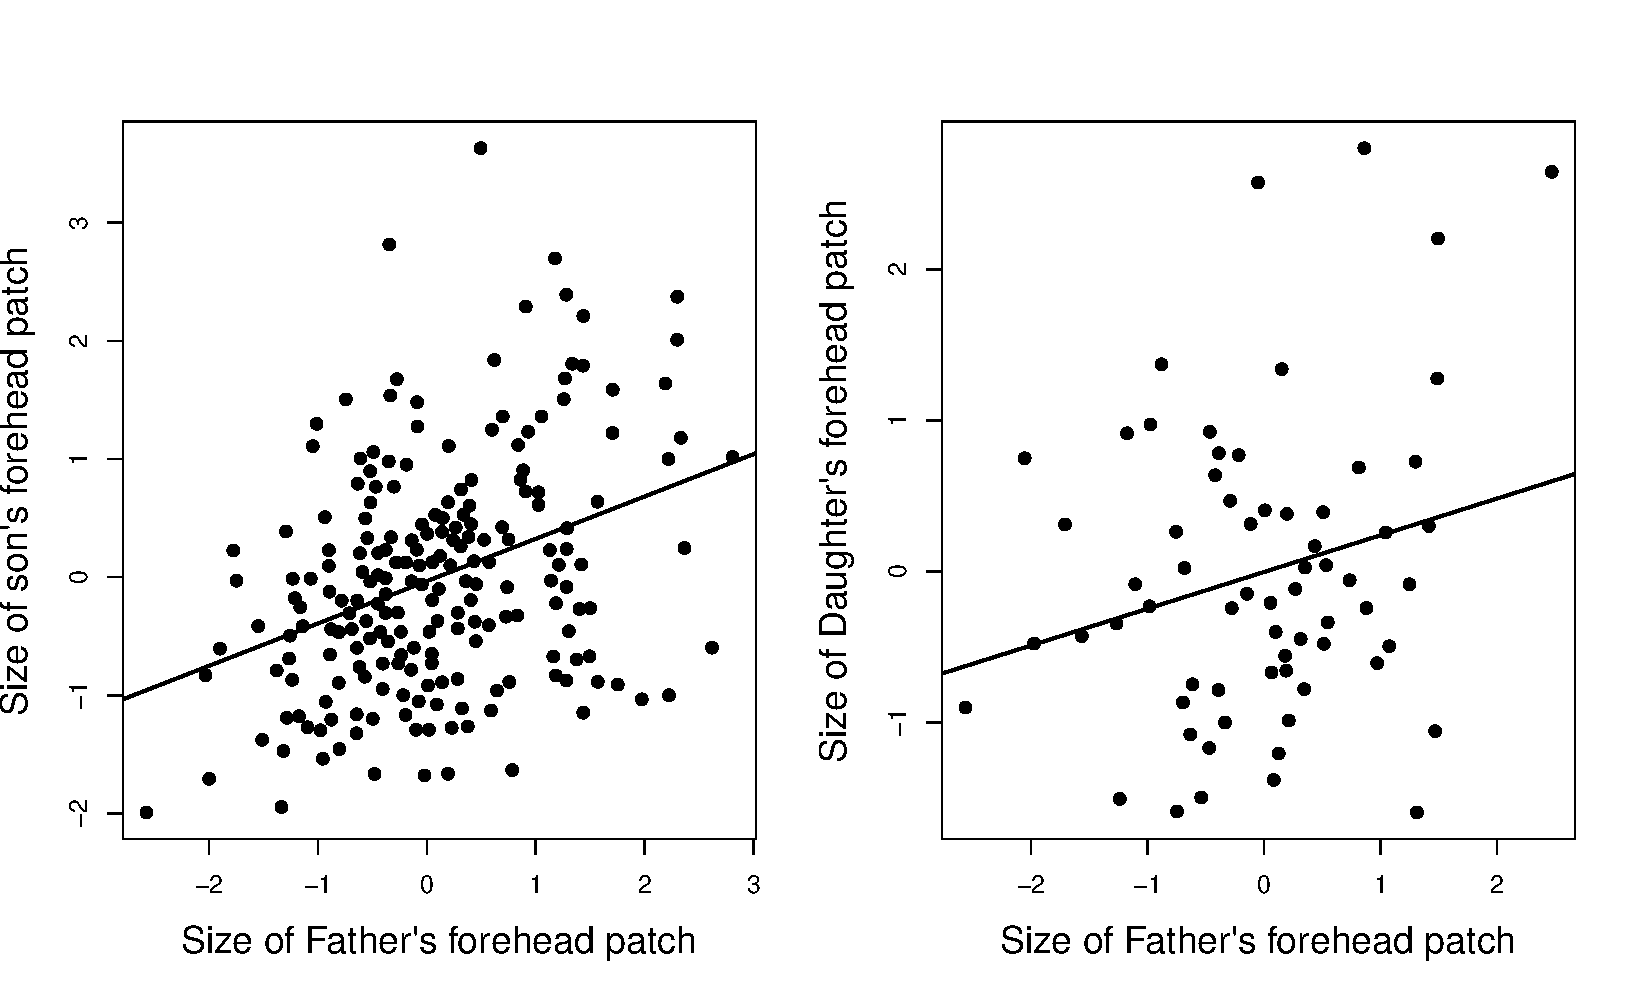
\includegraphics[width= \textwidth]{Journal_figs/Quant_gen/pied_fly_catcher_sex_genetic_corr/FlyCatcher_genetic_corr.pdf}
\end{center}
\caption{Relationship of standardized forehead patch size between
  farthers and sons and daughters in  Pied fly-catchers. Redrawn from \citeauthor{potti:11}.} \label{fig:FlyCatcher_genetic_corr}   %\cite{potti:11} 
\end{figure}

\begin{marginfigure}[-40mm]
\begin{center}
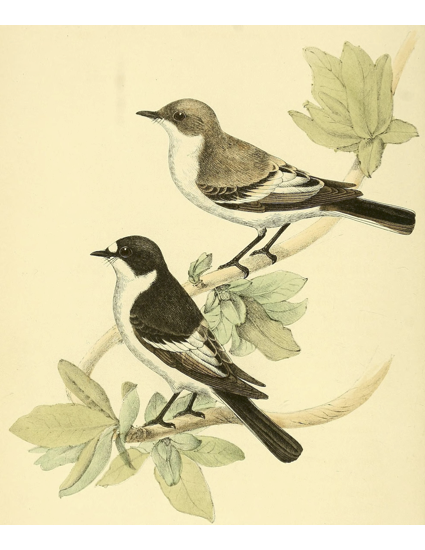
\includegraphics[width=0.9 \textwidth]{illustration_images/Quant_gen/pied_fly_catcher/pied_fly_catcher.pdf}
\end{center}
\caption{{\it Ficedula hypoleuca}, Pied fly-catcher.  Coloured illustrations of British birds, and their eggs.
London :G.W. Nickisson,1842-1850. BHL} \label{fig:FlyCatcher}   %% not
                                %% sure if it's a female or juv. https://www.biodiversitylibrary.org/page/40246319#page/334/mode/1up
\end{marginfigure}


\subsection{Non-additive variation.}

Up to now we've assumed that our alleles contribute to our phenotype in an
additive fashion. However, that does not have to be the case as there may be
non-additivity among the alleles present at a locus (\emph{dominance}) or among
alleles at different loci (\emph{epistasis}). We can accommodate these complications
into our models. We do this by partitioning our total genetic variance into
independent variance components.




%, such that the phenotype of the genotype of the heterozyote is the
%same as the $11$ homozygote. The area of each circle is proportion to the
%fraction of the population in each genotypic class ($p^2$, $2pq$, and $q^2$). 

\paragraph{Dominance.} To understand the effect of dominance lets consider how the allele
that a parent transmits influences their offspring's
phenotype. A parent transmits one of their two alleles at a locus to their offspring. 
Assuming that individuals mate at random, this allele is paired with another allele drawn at random from the population.
For example, if your mother transmitted allele 1 to you: with probability $p$ it would be paired with another allele 1, and you would be a homozygote; and with probability $q$ it's paired with a 2 allele and you're a heterozygote.

%The first variance component is the variance due to
%the additive contribution of each allele ($V_A$). 

Consider autosomal biallelic locus $\ell$, with frequency $p$ for allele 1, and
genotypes $0$, $1$, and $2$ corresponding to how many copies of allele
1 individuals carry. We'll denote the mean phenotype of an individual
with genotype $0$, $1$, and $2$ are $\overline{X}_{\ell,0}$,
$\overline{X}_{\ell,1}$, $\overline{X}_{\ell,2}$ respectively. Here this mean is
taken over all the environments and genetic backgrounds the alleles
are present on. We'll mean center (MC)
these phenotypic values setting $\overline{X}'_{\ell,0} = \overline{X}_{\ell,0} - \mu$, and
likewise for the other genotypes. 

We can think about the average
(marginal) MC
phenotype of an individual who received an allele 1 from their as the average of the MC phenotype
for heterozgotes and 11 homozygotes weighted by the probability that
an allele $1$ in present in these genotypes
\begin{equation} 
  a_{\ell, 1} = p\overline{X}'_{\ell,2}  + q\overline{X}'_{\ell,1},
\end{equation}
Similarly if your parent transmitted a 2 allele to you, your average
MC phenotype would be
\begin{equation}
  ~~ a_{\ell, 2} = p\overline{X}'_{\ell,1}  + q\overline{X}'_{\ell,0} 
\end{equation}

%the marginal value for allele 1, $a_{\ell, 1}$,  follows from the fact that (assuming HW) an allele 1 will be
%paired with another allele 1 with probability $p$, resulting in a
%genotype $11$ (with phenotypic deviation $\overline{X}'_{\ell,2}$) and will
%be paired with an allele 2 with probability $q$ in a heterozygote
%(with phenotypic deviation $\overline{X}'_{\ell,1}$). A similar argument
%can be made for $a_{\ell, 2}$. \\

%The additive MC genetic values (breeding values) of genotype 0, 1, and
%2 are then

Lets now consider the average phenotype of an offspring of each of our
three genotypes
\begin{center}
\begin{tabular}{cccc}
genotype: & 0, & 1, & 2.\\
additive genetic value: & $a_{\ell,2}+ a_{\ell,2}$, & $a_{\ell,1}+a_{\ell,2}$, & $a_{\ell,1}+a_{\ell,1}$   \label{add_values}
\end{tabular}
\end{center}
%
i.e. mean phenotype of each genotypes' offspring
averaged over across all possible matings to other individuals in the
population (assuming individuals mate at random). Theses are the
additive MC genetic values (breeding values) of our genotypes. 
Here we are simply adding up the additive contributions of the alleles present
in each genotype. These are the genotypic values of the trait that would result
taking only the additive effects of the components of the genotype.  

\begin{figure}
\begin{center}
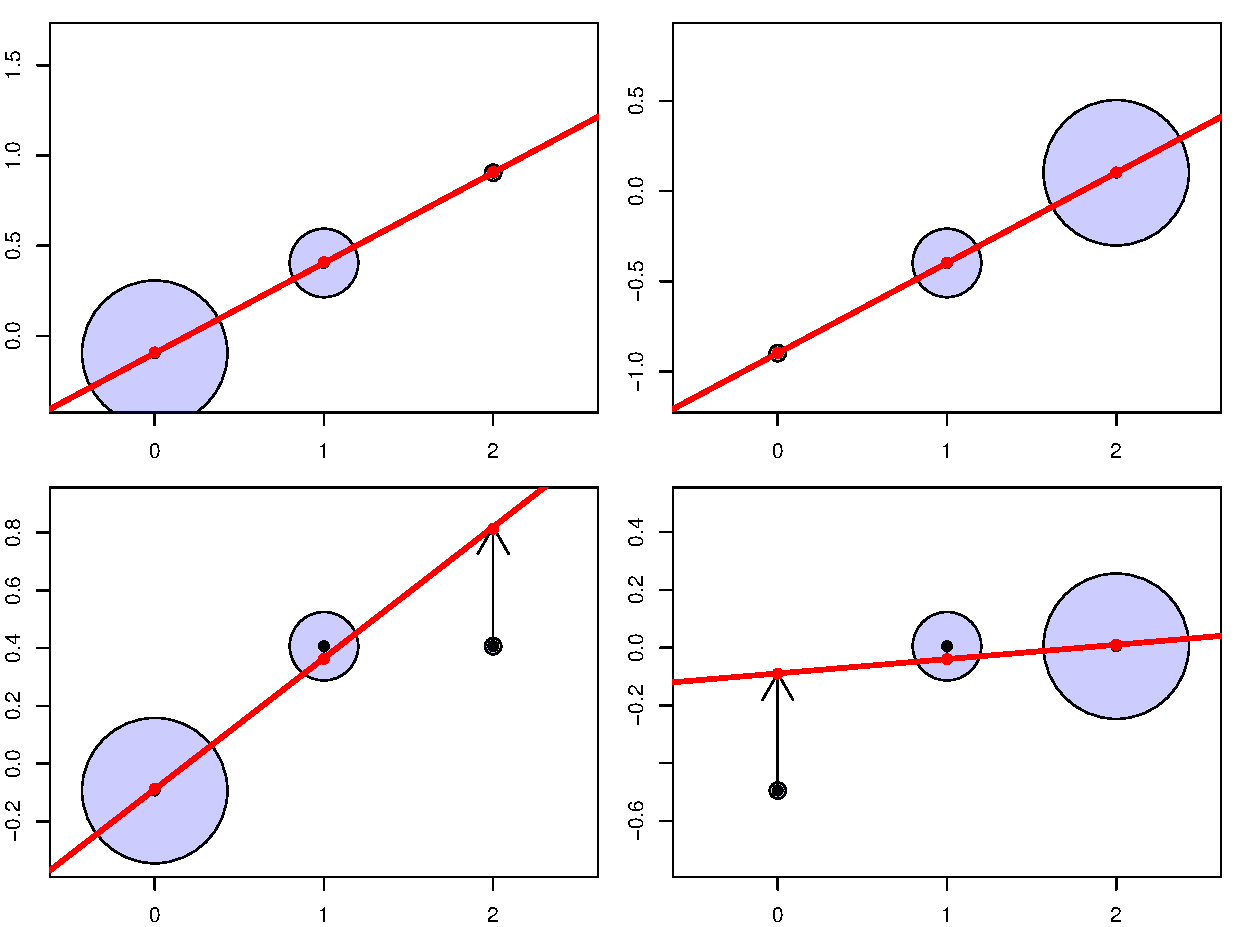
\includegraphics[width=\textwidth]{figures/additive_effect.pdf}
\end{center}
\caption{The average mean-centered (MC) phenotypes of each genotype. 
{\bf Top Row:} Additive relationship between genotype and phenotype. 
{\bf Bottom Row:} Allele 1 is dominant over allele 2, such that the
heterozygote has the same phenotype as the $22$ genotype ($2$). 
The area of each circle is proportion to the fraction of
the population in each genotypic class ($p^2$, $2pq$, and $q^2$). 
One the left column $p=0.1$ and the right column is $p=0.9$.
The additive genetic values of the genotypes are shown as
  red dots. The regression between phenotype and additive genotype is
  shown as a red line. The black vertical arrows show the difference
between the average MC phenotype and additive genetic value for each genotype. } \label{fig:add_dom}
\end{figure}


To illustrate this in Figure \ref{fig:add_dom} we plot two different cases of dominance
relationship, in the top row an additive polymorphism and in the second
row a fully dominant allele. The additive genetic values of the genotypes are shown as red dots. Note that the additive values of the genotypes line up with
the observed MC phenotypic means in the top row when our alleles interact in a
completely additive manner. Our additive genetic values always fall along a
linear line (the red line in our figure). The additive values are falling best
fitting line of linear regression for our population, when phenotype is
regressed against the additive genotype ($0$, $1$, $2$ copies of allele 1)
across all individuals in our population. Note in the dominant case the
additive genetic values differ from the observed phenotypic means, and are
closer to the observed values for the genotypes that are common in the
population. \\

The difference in the additive effect of the two alleles $a_{\ell, 2}-a_{\ell,
1}$ can be interpreted as a average effect of swapping an allele 1 for an
allele 2, we'll call this difference $\alpha_{\ell}=a_{\ell, 2}-a_{\ell, 1}$.
Our $\alpha_{\ell}$ is also the slope of the regression of genotype against
phenotype (the red line in Figure \ref{fig:add_dom}). Note that the slope of
our regression of genotype on phenotype ($\alpha_{\ell}$) does not depend on
allele frequency for our completely additive locus (top row of
\ref{fig:add_dom}). In contrast, when there is dominance, our the slope between
genotype on phenotype ($\alpha_{\ell}$) is a function of allele frequency
(bottom row of \ref{fig:add_dom}). When a dominant allele (1) is rare there is
a strong slope of genotype on phenotype, bottom left Figure \ref{fig:add_dom}.
This strong slope is because replacing a single copy of the 2 allele with a 1
allele in an individual has a big effect on average phenotype, as it will most
likely move an individual from being a 22 homozygote to being a 12
heterozygote. However, when the dominant allele (1) is common in the
population, replacing a 2 allele by a 1 allele in an individual on average has
little phenotypic effect. This small effect is because as we are mainly turning
heterozygotes into homozygotes (11), who have the same mean phenotype.  \\


\begin{marginfigure}
\begin{center}
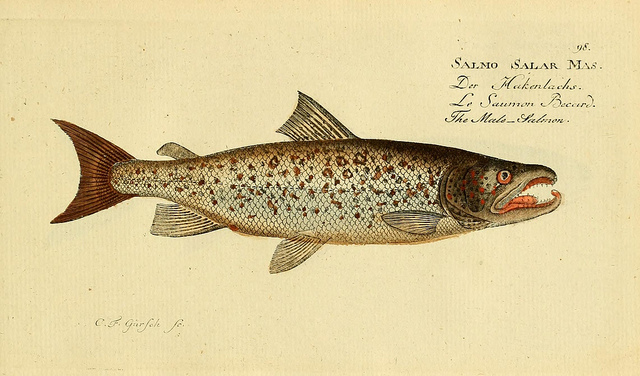
\includegraphics[width=\textwidth]{illustration_images/Quant_gen/Salmon/6918368208_5353868a88_z.jpg}
\end{center}
\caption{Atlantic Salmon ({\it Salmo salar}). Histoire naturelle des poissons. 1796. Bloch, M. E.} \label{fig:Salmon}
\end{marginfigure}


As as an example of this lets consider the genetics of sexual maturity
in Atlantic Salmon. \graham{finish}

\begin{figure}
\begin{center}
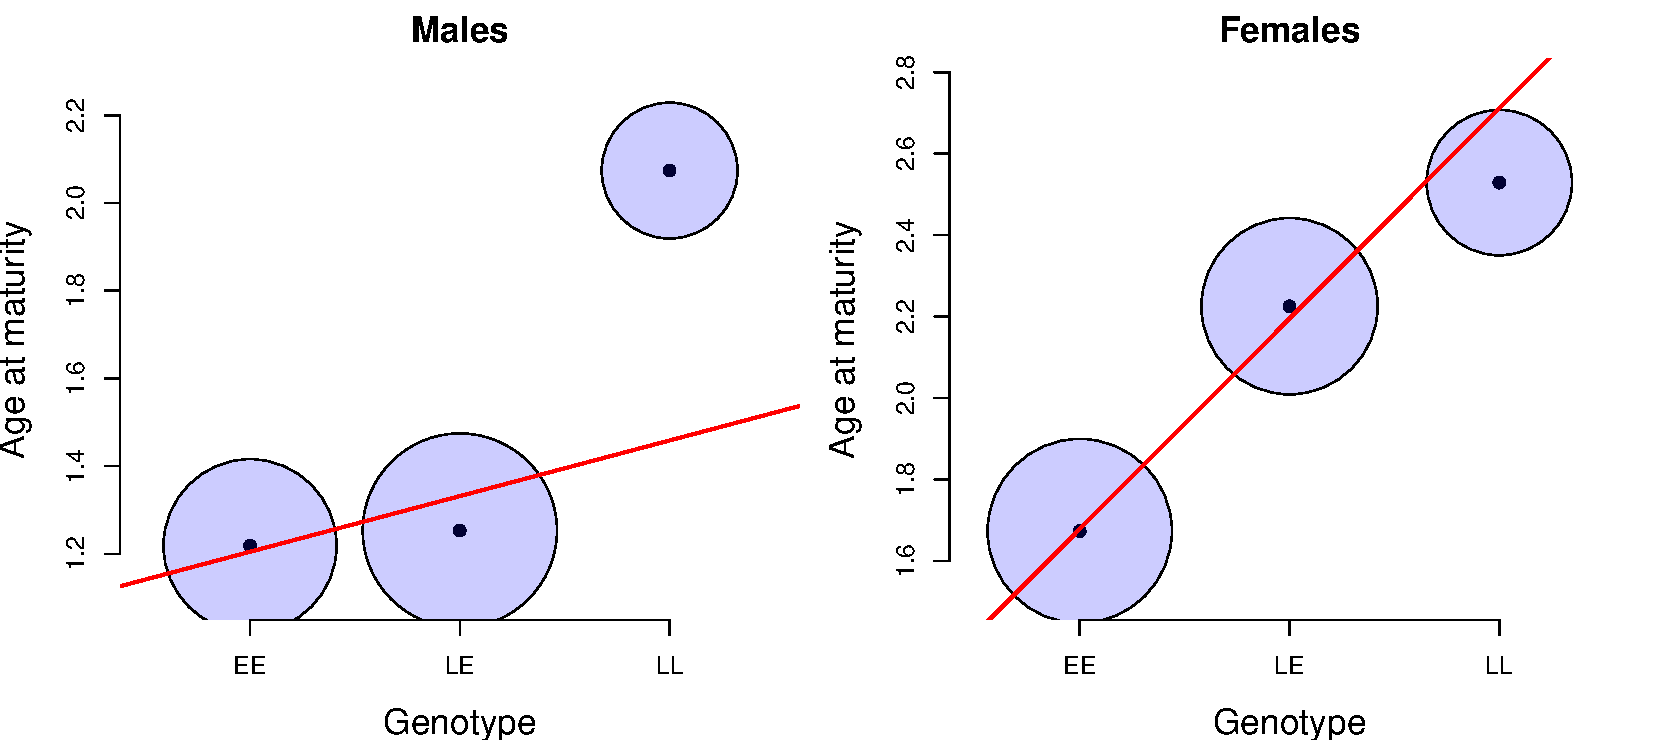
\includegraphics[width=\textwidth]{Journal_figs/Quant_gen/salmon_age/Salmon_age_dom.pdf}
\end{center}
\caption{The average age at sexual maturity for each genotype, broken
  down by sex. 
The area of each circle is proportion to the fraction of
the population in each genotypic class. The regression between phenotype and additive genotype is
  shown as a red line. The black vertical arrows show the difference
between the average MC phenotype and additive genetic value for each genotype. } \label{fig:salmon_add_dom}
\end{figure}

The variance in the population phenotype due to these
additive breeding values at locus $\ell$ assuming HW proportions is
\begin{align}
V_{A, \ell} &= p^2 (2a_{\ell,2})^2 + 2pq (a_{\ell,1}+a_{\ell,1})^2 + q^2
(2a_{\ell,0})^2 \nonumber \\
& = 2(p a_{\ell, 1}^2 + q a_{\ell, 2}^2 ) \nonumber \\
& = 2pq \alpha_{\ell}^2
\end{align}
The total additive effect can
be found by summing this additive genetic variance across loci
\begin{equation}
V_A = \sum_{\ell=1}^{L} V_{A, \ell} = \sum_{\ell=1}^{L}
2p_{\ell}q_{\ell} \alpha_{\ell}^2.
\end{equation}

Having assigned the additive genetic variance to be the variance
explained by the additive contribution of the alleles at a locus, we
define the dominance variance as the population variance among
genotypes at a locus due to their deviation from additivity.
We can calculate how much each genotypic mean deviates away from its
additive prediction at locus $\ell$ (the length of the arrows in
Figure \ref{fig:add_dom}), for example the heterozygote deviates 
\begin{equation}
d_{\ell,1} =\overline{X}'_{\ell,1}  - (a_{\ell,1}+ a_{\ell,2})
\end{equation}
away from its additive genetic value, with similar expressions for
each of the homozygotes ($d_{\ell,0}$ and $d_{\ell,2}$). We can then write the dominance variance at
our locus as the genotype-frequency weighted sum of our squared
dominance deviations
\begin{equation}
V_{D,\ell} = p^2 d_{\ell,0}^2+ 2pq d_{\ell,1}^2+ q^2 d_{\ell,2}^2.
\end{equation}
Writing our total dominance variance as the sum across loci 
\begin{equation}
V_D = \sum_{\ell=1}^{L}  V_{D,\ell}. 
\end{equation}
Having now partitioned all of the genetic variance into additive and
dominant terms, we can write our total genetic variance as 
\begin{equation}
V_{G} = V_A+V_D.
\end{equation}
We can do this because by construction the covariance between our
additive and dominant deviations for the genotypes is zero. We can
define the narrow sense heritability as before
$h^2=V_A/V_P=V_A/(V_G+V_E)$, which is the proportion of phenotypic
variance due to additive genetic variance. We can also define the 
total proportion of the phenotype variance due to genetic differences
among individuals, as the broad-sense heritability $H^2 =
V_G/(V_G+V_E)$. \\

\begin{table}
\begin{center}
\begin{tabular}{| l | c|}
\hline
Relationship (i,j)$^{*}$ &  $Cov(X_i,X_j)$  \\
\hline
parent--child & $\nicefrac{1}{2} V_A$\\
full siblings &$\nicefrac{1}{2} V_A +\nicefrac{1}{4} V_D$\\
identical (monzygotic) twins & $V_A+V_D$ \\
$1^{st}$ cousins & $\nicefrac{1}{8} V_A$\\
\hline
\end{tabular}
\end{center}
\caption{Phenotypic covariance between some pairs of relatives,
  include the dominance variation. $^{*}$Assuming this is the only relationship
the pair of individuals share (above that expected from randomly
sampling individuals from the population). } % doesn't this implicitly assume an infinite population?
\label{table:domcovar}
\end{table}

When dominance is present in the loci influencing our trait ($V_D>0$), we need to modify our
phenotype covariance among relatives to account for this
non-additivity. Specifically our equation for the covariance among a
general pair of relatives
(eqn. \ref{additive_covar_general_rellys} for additive variation) becomes
\begin{equation}
 Cov(X_1,X_2) = 2 F_{1,2} V_A + r_2 V_D
\end{equation}
where $r_2$ is the probability that the pair of individuals share 2
alleles identical by descent, making the same assumptions (other than additivity) that we made in deriving
eqn. \ref{additive_covar_general_rellys}.  In table
\ref{table:domcovar} we show the phenotypic covariance for some common
pairs of relatives. The regression of offspring phenotype on parental
midpoint still has a slope $V_A/V_P$. 

Full sibs and parent-offspring have the same
covariance if there is no dominance variance (as they have the same
kinship coefficient $F_{1,2}$). However, when dominance
is present ($V_D>0$), full-sibs resemble each other more than
parent-offspring pairs. That's because parents and offspring share
precisely one allele, while full-sibs can share both alleles (i.e. the
full genotype at a locus) identical by descent. We can attempt to
estimate $V_D$ by comparing different sets of relationships. For
example non-identical twins (full sibs born at same time) 
should have $1/2$ the phenotypic covariance of identical twins if
$V_D=0$. Therefore, we can attempt to estimate $V_D$ by looking at
whether identical twins have more than twice the phenotypic covariance
than non-identical twins. \\

The most important aspect of this discussion for thinking about
evolutionary genetics is that the parent-offspring covariance is still
only a function of $V_A$. This is because our parent (e.g. the mother) transmits only a
single allele, at each locus, to its offspring. The other allele the
offspring receives is random (assuming random mating), as it comes
from the other unrelated parent (the father). Therefore, the average
effect on the offspring phenotype of
the allele the offspring receives from the mother, is averaged over
the random allele the child receives from the father. Thus we only
care about the additive effect of the allele, as parents transmit only
alleles not genotypes to their offspring. This means that the short-term response
to selection, as described by the breeder equation, depends only on
$V_A$ and the additive effect of alleles. Therefore, if we can
estimate the narrow-sense heritability we can predict the short-term response.
However, if alleles display dominance our value of $V_A$ will change
as our loci change frequency, e.g. as dominant alleles become common
in the population their contribution to $V_A$ decreases. Therefore,
our value of $V_A$ will not be a constant across generations.

Up to this point we have only considered
dominance and not epistasis. However, we include epistasis in a
similar manner (for example among pairs of loci). This gets a little
tricky to think about so we will only briefly explain it. 
 We can first estimate the additive effect of the
alleles by considering the effect of the alleles averaging over the
other alleles they are paired with, just as before. We can then
calculate the additive genetic variance from this. We can estimate
the dominance variance, by calculating the residual variance among
genotypes at a locus unexplained by the additive effect of the
loci. We can then estimate the epistatic variance by estimating the
residual variance left unexplained among the two locus genotypes from the additive and dominant
deviations calculated from each locus separately. In practice these
high variance components are hard to estimate, and usually small as
much of our variance is assigned to the additive effect.  Again we
would find that we mostly care about $V_A$ for predicting short-term
evolution, but that the contribution of loci to the additive genetic
variance will depend on the epstatic relationships among loci.


\begin{question}
You collect observations of red deer within a generation; recording an
individual’s number of offspring and phenotypes, which are known to
have additive genetic variation, and construct the plots shown in
Figure \ref{fig:red_deer_Q} (standardizing the phenotypes). Answer the following
questions. For each question choose one of the bold options. Briefly justify each of your answers with reference to the breeder's
equation and multi-trait breeder's equation. No calculations are required. \\
{\bf A)}	Looking at just at figure \ref{fig:red_deer_Q} A, in what direction do you expect male antler size to evolve? \\
{\bf Insufficient information, increase, decrease.}\\

{\bf B)}	Looking just at figures \ref{fig:red_deer_Q} B and C, in what direction do you expect male antler size to evolve? \\
{\bf Insufficient information, increase, decrease.}\\

{\bf C)}	(3 Points) Looking at figures \ref{fig:red_deer_Q} A, B, and C in what direction do you expect male antler size to evolve? \\
{\bf Insufficient information, increase, decrease.}\\
\end{question}

\begin{figure}
\begin{center}
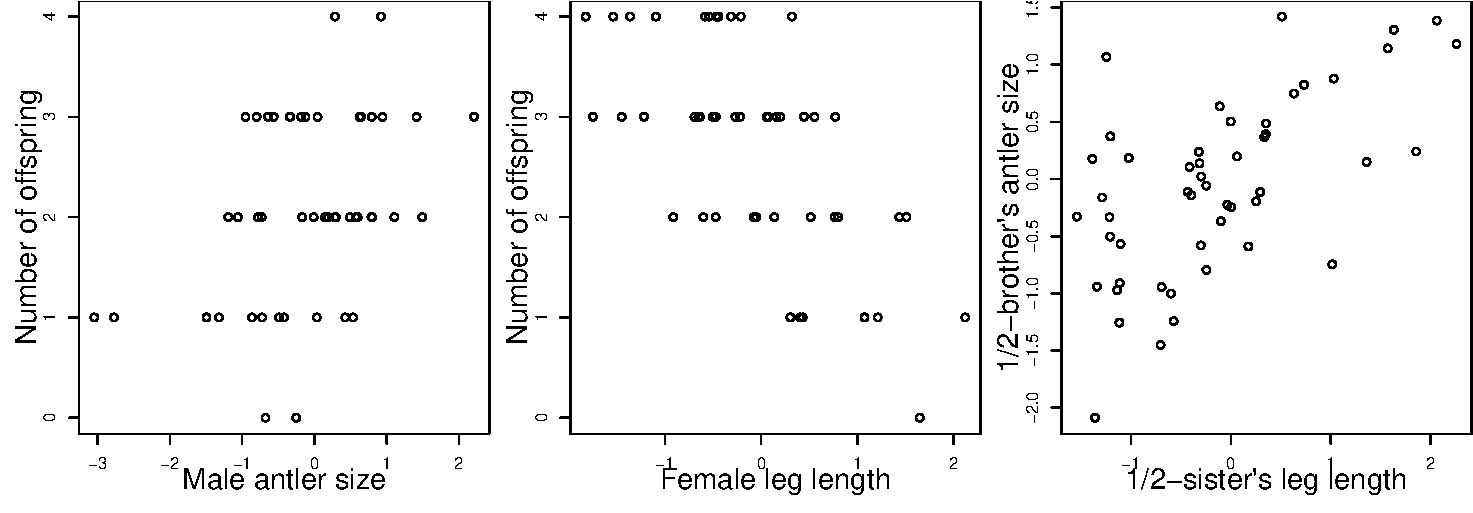
\includegraphics[width=\textwidth]{figures/Red_deer_selection.pdf}
\end{center}
\caption{ Observations of red deer within a generation; recording an
individual’s number of offspring and phenotypes, which are known to
have additive genetic variation. The figures left to right are A-C.} \label{fig:red_deer_Q}
\end{figure}



\begin{question}
How could you use 1/2 sibs vs full-sibs to estimate $V_D$? Why might
this be difficult in practice? Why are identical vs non-identical
twins better suited for this?
\end{question}

\begin{question}
Can you construct a case where $V_A=0$ and $V_D>0$? You need
just describe it qualitatively, you don't need to work out the
math. (tricker question).
\end{question}


\newpage
